%
% irreduzibel.tex
%
% (c) 2021 Prof Dr Andreas Müller, OST Ostschweizer Fachhochschule
%
\begin{frame}[t]
\frametitle{Irreduzible Markovkette}
\vspace{-20pt}
\begin{columns}[t,onlytextwidth]
\begin{column}{0.48\textwidth}
\begin{center}
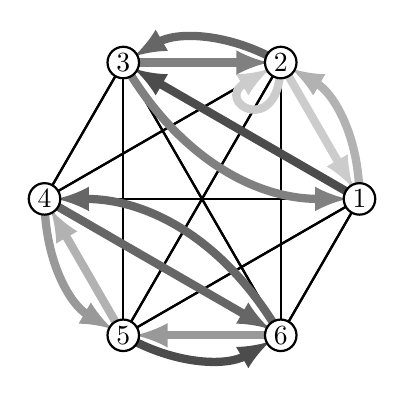
\begin{tikzpicture}[>=latex,thick]
\def\r{2}
\coordinate (A) at ({\r*cos(0*60)},{\r*sin(0*60)});
\coordinate (B) at ({\r*cos(1*60)},{\r*sin(1*60)});
\coordinate (C) at ({\r*cos(2*60)},{\r*sin(2*60)});
\coordinate (D) at ({\r*cos(3*60)},{\r*sin(3*60)});
\coordinate (E) at ({\r*cos(4*60)},{\r*sin(4*60)});
\coordinate (F) at ({\r*cos(5*60)},{\r*sin(5*60)});

\uncover<-2>{
\draw (A) -- (B);
\draw (A) -- (C);
\draw (A) -- (D);
\draw (A) -- (E);
\draw (A) -- (F);

\draw (B) -- (A);
\draw (B) -- (C);
\draw (B) -- (D);
\draw (B) -- (E);
\draw (B) -- (F);

\draw (C) -- (A);
\draw (C) -- (B);
\draw (C) -- (D);
\draw (C) -- (E);
\draw (C) -- (F);

\draw (D) -- (A);
\draw (D) -- (B);
\draw (D) -- (C);
\draw (D) -- (E);
\draw (D) -- (F);

\draw (E) -- (A);
\draw (E) -- (B);
\draw (E) -- (C);
\draw (E) -- (D);
\draw (E) -- (F);

\draw (F) -- (A);
\draw (F) -- (B);
\draw (F) -- (C);
\draw (F) -- (D);
\draw (F) -- (E);
}

\uncover<3->{

\draw[->,color=black!30,shorten >= 0.15cm,line width=3pt] (A) to[out=90,in=-30] (B);
\draw[->,color=black!70,shorten >= 0.15cm,line width=3pt] (A) -- (C);
\draw[->,color=black!20,shorten >= 0.15cm,line width=3pt] (B) -- (A);
\draw[->,color=black!60,shorten >= 0.15cm,line width=3pt] (B) to[out=150,in=30] (C);
\draw[->,color=black!20,shorten >= 0.15cm,line width=3pt] (B) to[out=-90,in=-150,distance=1cm] (B);
\draw[->,color=black!50,shorten >= 0.15cm,line width=3pt] (C) to[out=-60,in=180] (A);
\draw[->,color=black!50,shorten >= 0.15cm,line width=3pt] (C) -- (B);

\draw[->,color=black!40,shorten >= 0.15cm,line width=3pt]
	(D) to[out=-90,in=150] (E);
\draw[->,color=black!30,shorten >= 0.15cm,line width=3pt]
	(E) -- (D);
\draw[->,color=black!70,shorten >= 0.15cm,line width=3pt]
	(E) to[out=-30,in=-150] (F);
\draw[->,color=black!40,shorten >= 0.15cm,line width=3pt]
	(F) -- (E);
\draw[->,color=black!60,shorten >= 0.15cm,line width=3pt]
	(F) to[out=120,in=0] (D);
\draw[->,color=black!60,shorten >= 0.15cm,line width=3pt]
	(D) -- (F);
}

\fill[color=white] (A) circle[radius=0.2];
\fill[color=white] (B) circle[radius=0.2];
\fill[color=white] (C) circle[radius=0.2];
\fill[color=white] (D) circle[radius=0.2];
\fill[color=white] (E) circle[radius=0.2];
\fill[color=white] (F) circle[radius=0.2];

\draw (A) circle[radius=0.2];
\draw (B) circle[radius=0.2];
\draw (C) circle[radius=0.2];
\draw (D) circle[radius=0.2];
\draw (E) circle[radius=0.2];
\draw (F) circle[radius=0.2];

\node at (A) {$1$};
\node at (B) {$2$};
\node at (C) {$3$};
\node at (D) {$4$};
\node at (E) {$5$};
\node at (F) {$6$};

\end{tikzpicture}
\end{center}
\uncover<2->{%
\begin{block}{Irreduzibel}
Graph zusammenhängend $\Rightarrow$
Keine Zerlegung in Teilgraphen möglich
\end{block}}
\end{column}
\begin{column}{0.48\textwidth}
\uncover<3->{%
\begin{block}{Reduzibel}
Die Zustandsmenge zerfällt in zwei disjunkte Teilmengen $V=V_1\cup V_2$
und es gibt keine Übergängen zwischen den Mengen:
\uncover<4->{%
\begin{align*}
P
&=
\begin{pmatrix*}[l]
0  &0.2&0.5&   &   &   \\
0.3&0.2&0.5&   &   &   \\
0.7&0.6&0  &   &   &   \\
   &   &   &0  &0.3&0.4\\
   &   &   &0.4&0  &0.6\\
   &   &   &0.6&0.7&0  
\end{pmatrix*}
\end{align*}}%
\uncover<5->{%
$P$ zerfällt in zwei Blöcke die unabhängig voneinander analysiert werden können
}
\end{block}}
\end{column}
\end{columns}
\end{frame}
